\documentclass[conference]{IEEEtran}
\IEEEoverridecommandlockouts
% The preceding line is only needed to identify funding in the first footnote. If that is unneeded, please comment it out.
\usepackage{cite}
\usepackage{amsmath,amssymb,amsfonts}
\usepackage{algorithmic}
\usepackage{graphicx}
\usepackage{textcomp}
\usepackage{hyperref} 

\usepackage{xcolor}
\usepackage[section]{placeins}
\def\BibTeX{{\rm B\kern-.05em{\sc i\kern-.025em b}\kern-.08em
    T\kern-.1667em\lower.7ex\hbox{E}\kern-.125emX}}
\begin{document}

\title{Determining Most Important Features from Depression Survey Using Random Forest Classifier\\}

\author{\IEEEauthorblockN{1\textsuperscript{st} Nathan Pham}
\IEEEauthorblockA{\textit{College of Science} \\
\textit{California State Polytechnic University, Pomona}\\
Pomona, USA \\
nathanpham@cpp.edu}
\and
\IEEEauthorblockN{2\textsuperscript{nd} Roberto S. Toribio}
\IEEEauthorblockA{\textit{College of Science} \\
\textit{California State Polytechnic University, Pomona}\\
Pomona, USA\\
rstoribio@cpp.edu}

\and
\IEEEauthorblockN{3\textsuperscript{rd} Rida Siddiqui}
\IEEEauthorblockA{\textit{College of Science} \\
\textit{California State Polytechnic University, Pomona}\\
Pomona, USA\\
rsiddiqui@cpp.edu}
\and
\IEEEauthorblockN{4\textsuperscript{th} Ly Hoang}
\IEEEauthorblockA{\textit{College of Science} \\
\textit{California State Polytechnic University, Pomona}\\
Pomona, USA\\
lhrivera@cpp.edu}

}

\maketitle

\begin{abstract}
%(Questions for professor are in parenthesis)
Depression is a mental illness that causes persistent feelings of sadness and can have negative effects on one's thinking, behavior, and physical health. Because of these negative effects, we wanted to analyze some reasons that lead to depression. The dataset we chose has a total of 1429 instances and 23 attributes related to depression. Moreover, the class labels are binary, specifically, the labels are depression or no depression. This dataset came from a study about the living conditions of people living in rural zones in Siaya County, Kenya. Our objective was to identify which attributes from the dataset contribute the most to an individual developing depression. To do so, the Sklearn fitted attribute, feature importance was utilized to determine the most important features. The algorithm we used is the Random Forest classifier, while using a grid search to find the hyperparameters that maximize the F1-score. We found the top 5 most important features to be age, education level, no lasting investment, durable assets, and living expenses. Additionally, the importance of all features was visually represented using a bar graph. A confusion matrix was also created to help visualize the performance of our model.

\end{abstract}
\section{Introduction}
Depression is a mental illness that is characterized by deep and long-lasting feelings of sadness. Depression can negatively affect one's thinking, behavior, and physical health. Because of these negative effects on humans, we wanted to analyze some reasons that lead to depression such as marital state, education level, and financial state. The dataset which we chose came from a study done regarding depression in 2015 in rural Siaya County in Western Kenya. the dataset consists of 23 features and 1429 samples. Our objective was to identify which attributes from the chosen dataset contribute the most to an individual developing depression. To achieve this, we used a Random Forest Classifier and adjusted its hyperparameters via a grid search to create a model that has the highest F1-score.



\section{Dataset}

\subsection{Dataset Background}
The dataset which was used analyzes factors that contribute to depression. It has 23 features and 1429 samples. This dataset came from a 2015 study conducted by the Busara Center in rural Siaya County, near Lake Victoria in western Kenya [1]. Some attributes are age, number of children, education level, total family members, and living expenses. The class labels are binary. Specifically, the label is either "has depression" (positive) or "no depression" (negative). There are 238 positive labels and 1191 negative labels. The ratio of positive to negative labels is 19.98\%, showing that the dataset has a moderate class imbalance.


\subsection{Feature Description}
\begin{figure}[hbt!]
\centering
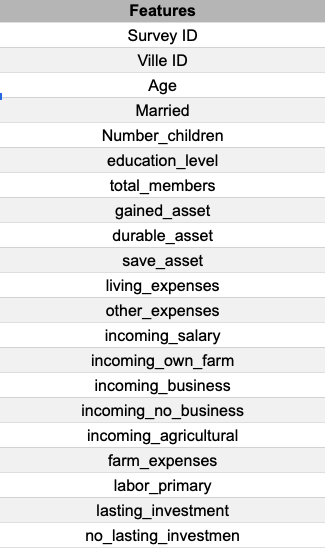
\includegraphics[width=30mm]{feat.png}
\caption{Features from the dataset\label{overflow}}
\end{figure}
Although most features are self-explanatory,there are some features which deserve an explanation. The first of these is no lasting investment, which are investments that are easily converted to cash, such as short-term bonds. On the other hand, durable assets are those assets which are capable of generating flows of goods and services. This is exemplified by computers, tools, and even livestock. All features are listed in Figure 1.


\subsection{Data Exploration}
Figure 2 shows that the dataset has a class imbalance. There are 83.3\% of individuals with no depression and 16.7\% of individuals with depression. As a consequence, F1-score was used as the metric to evaluate the model. Using accuracy is misleading since a naive prediction that an individual has no depression will yield an accuracy of 83.3\%.
\begin{figure}[hbt!]
\centering
\includegraphics[width=50mm]{class_dist.png}
\caption{Class Proportion\label{overflow}}
\end{figure}

The disproportion of males to females in the survey data is also worth highlighting. The dataset consists of 91.8\% females and 8.2\% males, shown in Figure 3. This decreases the generality of the model since males are highly underrepresented.
\begin{figure}[hbt!]
\centering
\includegraphics[width=50mm]{m_to_f_ratio.png}
\caption{Gender Proportion\label{overflow}}
\end{figure}

\begin{figure}[ht!]
\centering
\includegraphics[width=85mm]{corre_mat.png}
\caption{Feature Correlation Matrix\label{overflow}}
\end{figure}

A correlation matrix was used to gauge the correlation between different features. On inspection, there appears to be a very modest correlation between age and depression. Some other features that are correlated with depression to an even smaller degree include total family members, durable assets, and no lasting investments. The correlation matrix that was generated can be seen in Figure 4.


\subsection{Data Processing}
From the Data exploration process, it was determined that all feature values within the dataset were numerical. So, in terms of encoding, there were no major changes made to the dataset. However, some missing values were present. The missing values were limited to the feature no lasting investment, and to fix this issue the median value was used. The median was used to fill in the 20 missing values that were present within this feature's column. The features Survey id and Ville id were also dropped for our purposes.


\section{Methodology}
A Random Forest Classifier was used for classification purposes. The Random Forest algorithm can be used in both classification and regression problems, and consists of many decision trees, each of which gives some results. This algorithm gives better results when there are higher number of trees in the forest, which prevents the model from overfitting.  

Random Forest ensures that the behavior of each tree is not too correlated with the behavior of any of the other trees in the model through Bagging (Bootstrap Aggregation). Decisions trees are very sensitive to the dataset, meaning that small changes to the training set can result in significantly different models. Random Forest uses this to its advantage by allowing each tree to randomly sample from the dataset with replacement, resulting in different trees. These trees are then merged to get a more accurate and stable prediction.


To have a baseline to compare to, a naive implementation of the model was used. Moreover, Stratified $k$-fold cross validation was used. Seeing the effect that different values had on the F1-score of the naive model, helped in setting a range to the values of the hyperparameters for the general model. This naive model yielded an F1-score of 4.6\% The hyperparameters used for this model can be seen in Figure 5.
\begin{figure}[hbt!]
\centering
\includegraphics[width=60mm]{baseline.png}
\caption{Hyperparameter values for baseline model\label{overflow}}
\end{figure}


For the general model validation purposes Stratified $k$-fold was used with a $k$ value of 10. This specific value of $k$ was picked because it has been found through experimentation to generally result in a model skill estimate with low bias and modest variance. The reason why Stratified $k$-fold was used as the validation technique is because it ensures that the training and test sets have the same proportion of class labels as the original dataset. This is desirable due to the class imbalance that exists within the dataset.

\begin{figure}[hbt!]
\centering
\includegraphics[width=60mm]{hyperparams.png}
\caption{Hyperparameters and their values
\label{overflow}}
\end{figure}
A grid search was conducted in order to tune the hyperparameters listed in Figure 6. As mentioned, the values to test were determined from some trial runs of the baseline model. One hyperparameter we found to be quite important was class weight. This hyperparameter helps manage the weights associated with each class. When we weren't using this hyperparameter, both of the classes were being assigned weight one, which wasn't helpful since the dataset has a class imbalance. After adding class weight to the list of hyperparameters, the F1-score got better.

It is worth mentioning that after determining the best hyperparameters from the grid search, the model was trained again using these values of the hyperparameters. Then after completing this second training/testing phase, the model was used to determine the most important features.

To determine the most important features from the model we used a fitted attribute from the Sklearn library called feature importances. This attribute is computed as the mean and standard deviation of accumulation of the impurity decrease with each tree. 

This second training/testing phase also was utilized to determine a confusion matrix for validation purposes. During this phase, Stratified K-fold validation was used once again.

After using a Random Forest Classifier, while using a grid search and K-fold cross validation, the highest F1-score came out to 27.7\%. This is a noteable improvement from the baseline classifier, which had an F1-score of 4.6\%. 
The hyperparameter values that yielded the best F1-score are listed in Figure 7.

\begin{figure}[hbt!]
\centering
\includegraphics[width=60mm]{best_hyp.png}
\caption{Best hyperparameter values from Grid-Search \label{overflow}}
\end{figure}

\section{Results}

After training the model again using these hyperparameter values, we found the top features. The top 5 features were age, education level, no lasting investment, durable assets, and living expenses. Moreover, the complete ranking of all the features from most important to least important are visualized in Figure 8. 
\begin{figure}[hbt!]
\centering
\includegraphics[width=90mm]{fi.png}
\caption{Most Important Features ranked from most to least important\label{overflow}}
\end{figure}

These features being the most important was not surprising to see, despite the fact that we anticipated marital status and household size to be included within the top five features. Nonetheless, our intuition that economic state would be an important feature was not misguided. Although economic state is not directly a feature of the dataset, it can be implicitly represented by the features, education, no lasting investment, durable assets, and living expenses.


We created a confusion matrix to visualize the performance of the Random Forest classifier. As depicted in Figure 9, the model was unable to minimize false negatives and false positives. At the top right (false positive), the classifier marked 298 individuals as depressed, when they were actually healthy. And at the bottom left (false negative), the classifier marked 162 individuals as healthy, when they were actually depressed.
\begin{figure}[hbt!]
\centering
\includegraphics[width=90mm]{cm.png}
\caption{Confusion Matrix\label{overflow}}
\end{figure}

One reason why the F1-score was rather low was because of both the class imbalance and the size of the dataset, with only 1429 instances. If the dataset would have been a bit larger, then the F1-score could have possibly improved more. Nonetheless, our goal to find the most important features was achieved.


\section{Related Work}
The work  by Yevhen Strakhov [2] also used the same dataset. The major difference between Strakhov's work and our work is that he used a Logistic Regression model instead of a Random Forest Classifier. Another major difference is that he standardized features that are in an inconvenient scale. Some of the features that were standardized include gained assets, durable assets, and living expenses to name a few. Some similarities between Strakhov's research and our research was the use of a grid search to tune the hyperparameters of his model. Furthermore, he also used F1-score as the metric to optimize during the grid search. In terms of results, Strakhov was only able to improve the F1-score to 16.1 \%. On the other hand, our group was able to improve it to 27.7 \%, which is modestly better than what he achieved.

\section{Source code for Project Implementation and Latex Files}
All the relevant source code, as well as the proposal and final report latex files can be found at \url {https://github.com/robo27918/cs4210_finalProj.git}

\section{Conclusion}
Although we were unable to increase the F1-score substantially, there were many important lessons learned while going through the machine learning pipeline. We were able to get a good understanding of the dataset using various tools provided by the Pandas Library during the data exploration process. These insights were invaluable to ensure we made the correct choice in choosing the accuracy metric. Moreover, we were able to see the severity of our class imbalance and were able to address this issue by using both Stratified K-fold cross validation and the hyperparameter called class weight while implementing our Random Forest Classifier. Making these adjustments also allowed us to increase our knowledge of the Sklearn library and the machine learning pipeline. Another important thing we learned was the importance of having a large dataset. Having a larger dataset might have resulted in a better performance of the model and the number of false positives and false negatives might have been reduced. Regardless, the lessons learned here can be applied to a future dataset with more data instances. Furthermore, we could find a richer dataset without some of the issues that were discussed such as the low male-to-female ratio and class imbalance.



\begin{thebibliography}{00}
\bibitem{b1} Busara Center for Behavioral Economics, Busara Mental Health Prediction Challenge Dataset, Siaya County, Kenya: Busara Center for Behavioral Economics, 2015. [Online]. Available: https://www.kaggle.com/datasets/diegobabativa/depression [Accessed: October 15, 2020]
\bibitem{b2} Y. Stakhov, "Logistic regression" Kaggle, 19-Jul 2022.[Online]. Available :https://www.kaggle.com/code/emstrakhov/logisitc-regression notebook. [Accessed:16-Nov-2022].


\end{thebibliography}
\vspace{12pt}
\color{red}
\end{document}
